\documentclass[../Hovedrapport.tex]{subfiles}
\begin{document}
%\vspace{-30pt}

%------------------------------------------------------------------------------
% --------------------- Nedenstående er beregninger på systemet-------------
\section{Kompressorberegninger (N.J. \& M.N.)} 
    \label{sec:indledendeberegninger}
Dette afsnit indeholder beregninger af massestrømmen, som kompressoren leverer, samt den el-effekt den benytter for at kunne levere denne massestrøm. Hertil vil en kondenseringsydelse blive beregnet, der tager hensyn til en antaget varmestrøm for kølingen af kompressoren. Ydermere vil tabet i kompressoren blive beregnet sammen med effektfaktoren og slutteligt vil et log p,h-diagram blive udarbejdet. 
Beregningerne fremgår af appendiks \ref{sec:apndx_kompressorberegninger}.
%------------------------------------------------------------------------------
\subsection{Massestrøm i kompressor (N.J. \& M.N.)}
\label{sec:masse}
Ved udregning af massestrømmen i kompressoren  findes den teoretiske slagvolumen i databladet til $ V_s= 5,08\cdot 10^{-6} \si{m^3} $ jf. bilag \ref{sec:bil_kom}. Hertil omregnes omdrejningstallet på 4000 RPM til omdrejninger pr. sekund, herved fås $ n_k=66,67 \frac{1}{s} $. Den teoretiske slagvolumenstrøm kan nu udregnes ved følgende:
\begin{align}
    q_{V,s}=V_s \cdot n_k =0,339 \cdot 10^{-3} \si{\frac{m^3}{s}} 
\end{align}

Når volumenstrømmen i tilstand 1 skal findes i figur \ref{fig:Anlægsoversigt}, så benyttes den volumetriske virkningsgrad fra afsnit \ref{sec:virkgrad} multipliceret med den teoretiske slagvolumenstrøm.
\begin{align}
    q_{V,1}=V_s \cdot \eta_V = 0,233 \cdot 10^{-3} \si{\frac{m^3}{s}}
\end{align}
Ud fra volumenstrømmen fundet i ovenstående ligning kan massestrømmen findes ved densiteten i den givne tilstand til $\rho_1=10,42\si{\frac{kg}{m^3}}$ fra tabel \ref{tab:procesval}.
\begin{align}
    q_{mR}=q_{V,1} \cdot \rho_1 = 2,43\cdot 10^{-3} \SI{}{kg/s}
\end{align}
Det vil altså sige, at massestrømmen for kølemidlet vil være $2,43\cdot 10^{-3} \SI{}{kg/s}$.
%------------------------------------------------------------------------------
\subsection{El-effekt (N.J. \& M.N.)}
    \label{sec:eleffektudre}
Foruden massestrømmen kan el-effekten til kompressoren også findes under de givne forhold. Her kan el-effekten findes ud fra den tidligere fundne energibalance for kompressoren. I første omgang kan $P_{el}$ findes og hertil kan størrelsen af varmestrømmen for kølingen så bestemmes. 
\begin{align}
    P_{el}=q_{mR} \cdot \dfrac{h_{2s}-h_1}{\eta_{s,k}}=189,1 \si{\watt}
\end{align}
Når el-effekten er udregnet kan størrelsen af varmestrømmen for kølingen, $\Phi_{\text{køl}}$, tilnærmelsesvis findes ved at antage en kølingsgrad, $k_{\textit{ø}}$. Denne faktor er typisk mellem 0,1-0,3, hvor der i følgende beregning antages en værdi på $k_{\textit{ø}}=0,2$ \citep{termo}. Dette indsættes dermed i formlen:
\begin{align}
    \Phi_{\text{køl}}= k_{\textit{ø}} \cdot P_{el} = 37,83 \si{\watt}
\end{align}
%------------------------------------------------------------------------------
\subsection{Kondenseringsydelse (U.H. \& B.B.)}
    \label{sec:kondenseringsydelse_med_koling}
En tredje størrelse, der kan bestemmes når det kommer til køletekniske systemer, er kondenseringsydelsen. Denne ydelse beskriver, hvor stor en varmeafgivelse kompressoren kan sikre på kondensatorsiden. Entalpien $h_2$ bestemmes nu jf. energibalancen fra ligning \ref{eq:kompressorEB}, hvor der tages hensyn til køling af kompressoren.
\begin{align}
    h_2 = \frac{P_{el}-\Phi_{\text{køl}}}{q_{mR}}+h_1= \SI{463,0}{\frac{kJ}{kg}} 
\end{align}
Idet entalpien og trykket kendes, kan temperaturen findes ved opslag i EES, hvor denne temperatur bliver $t_2=\SI{84,82}{\celsius}$.

Ud fra energibalanceligningen for kondensatoren i ligning \ref{eq:kondensatorEB} kan kondenseringsydelsen isoleres, hvilket giver følgende:
\begin{align}
    \Phi_k=q_{mR}\cdot(h_2-h_3)=\SI{483,9}{\watt}
    \label{eq:kondenseringsydelse_udregnet}
\end{align}
%------------------------------------------------------------------------------
\subsubsection*{Tabet i kompressoren}
Den fundne massestrøm benyttes til at bestemme varmestrømmen $\Phi_{tab,1}$. Dette gøres ved følgende ligning:
 \begin{align}
    \Phi_{tab,1}=q_{mR}\cdot (h_2-h_{2s})=\SI{58,64}{\watt}
 \end{align}
  Nu er størrelsen på $\Phi_{tab,1}$ fundet. Det bør dog nævnes, at denne størrelse ikke vil være med i energibalancerne senere, hvilket skyldes, at entalpien $h_2$ vil blive benyttet i disse beregninger. Denne beregning er foretaget for at give et indblik i størrelsen af tabet i forhold til en perfekt isentropisk proces.

Desuden kan det kontrolleres, hvorvidt energibalancerne er rigtige ud fra ligning \ref{eq:helesystemEB} for hele systemet:
\begin{align}
   P_{el} +\Phi_0 +\Phi_{\textit{køl}} - \Phi_{tab}-\Phi_k = 0
\end{align}
Det kan i ovenstående ligning ses, at der er redegjort for alle effekterne, som overskrider systemgrænsen på hele anlægget. Disse varmestrømme fremgår også af figur \ref{fig:kun_sys}.
%------------------------------------------------------------------------------
\subsection{Effektfaktor og energiforbrug (N.J. \& M.N.)}
    \label{sec:effektfaktor_energiforbrug}
I et køleteknisk system er der visse parametre, som angiver, hvor godt køleanlægget opererer. Her angiver effektfaktoren, som også kaldes kølefaktoren og COP, forholdet mellem den tilførte energi, i form af varme fra fordamperen, og den tilførte el-effekt.
\begin{align}
\label{eq:effektfaktorulle}
    \epsilon_{\textit{køl}}= \dfrac{\Phi_0}{P_{el}} = 1,77
\end{align}
Hvis energiforbruget ønskes bestemt for en given tidsperiode, kan følgende formel benyttes:
\begin{align}
    E_{forbrug}=P_{el} \cdot \Delta t
\end{align}
%------------------------------------------------------------------------------
\subsection{Log p,h-diagram (U.H.. \& M.N.)}
    \label{sec:logphdiagram}
På baggrund af beregningerne i ovenstående underafsnit, er log p,h-diagrammet for køleanlægget optegnet via programmet \textit{Coolpack}\citep{Coolpack}, hvilket fremgår af figuren nedenfor. Her er de forskellige tilstandsstørrelser indtegnet, hvor tilstand 2 er vist for henholdsvis en ikke-kølet proces (se streg 1-2ik), en kølet proces (se streg 1-2) samt en isentropisk proces (se streg 1-2s).
\begin{figure}[H]
    \centering
    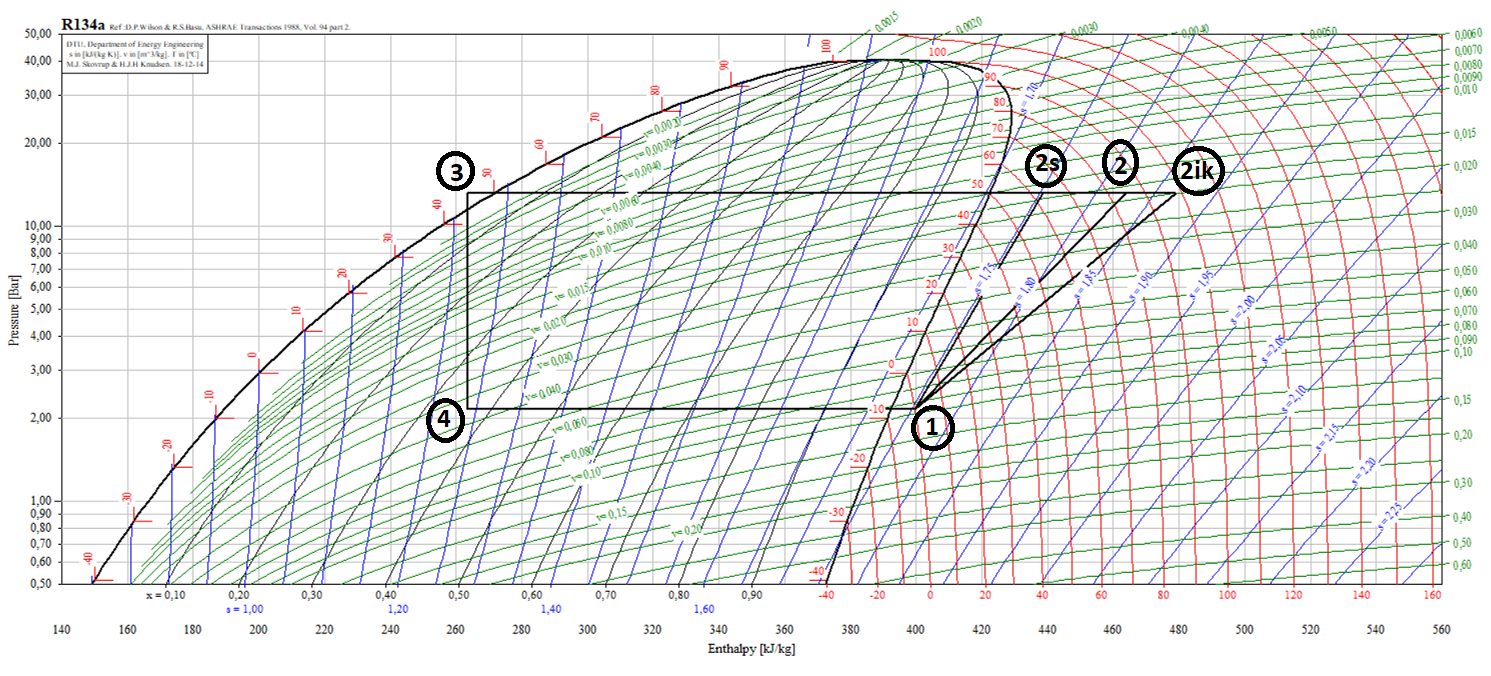
\includegraphics[width=1.0\textwidth]{Billeder/logPHdiagram.PNG}
    \caption{\textit{Log p,h diagrammet for køleanlægget med R134a som kølemiddel}}
    \label{fig:logphdiagram}
\end{figure}

Af figur \ref{fig:Anlægsoversigt} fremgår tilstandsstørrelsernes placering i anlægget. 
%------------------------------------------------------------------------------
\subsection{Delkonklusion (Alle)}
Der er nu fundet en massestrøm i køleanlægget til $q_{mR} = 2,43 \cdot 10^{-3} \SI{}{\frac{kg}{s}}$. Hertil er en el-effekt på $P_{el}=189,1 \si{W}$ blevet bestemt og ud fra dette er $\Phi_{\text{køl}}$ blevet bestemt til $37,83 \si{W}$ ved en antaget kølegrad på $0,2$. Der er ud fra denne $\Phi_{\text{køl}}$, $\eta_s$ og $P_{el}$ fundet en entalpi, $h_2$, til $463 \si{\frac{kJ}{kg}}$, hvorpå tabet i kompressoren kan bestemmes. Hertil kan de nyligfundne værdier sammenfattes i tabel \ref{tab:procesval_med_h2}:
\begin{table}[H] 
\renewcommand{\arraystretch}{1.4}
\centering
\vspace{-0.3cm}
\begin{tabular}{|c|c|c|c|c|}  \cline{1-5} \rowcolor[gray]{0.7}
\multicolumn{5}{|c|}{\textbf{Anlægstemperaturer}}      \\ \hline \rowcolor[gray]{.8}
\textbf{Proces} & \textbf{T}    & \textbf{P}    & \textbf{$\rho$}   & \textbf{h} \\ \hline 

	\textbf{1}                           & \SI{0}{\celsius}             & \SI{2,17}{\bar}     & \SI{10,41}{\frac{kg}{m^3}}        & \SI{400,7}{\frac{kJ}{kg}}       \\  \hline
	\textbf{2s}                          & \SI{63,02}{\celsius}            & \SI{13,18}{\bar}    & \SI{60,17}{\frac{kg}{m^3}}        &  \SI{438,9}{\frac{kJ}{kg}}    \\\hline
	\textbf{2}                           & \SI{84,82}{\celsius}         & \SI{13,18}{\bar}    & \SI{53,22}{\frac{kg}{m^3}}         & \SI{463,0}{\frac{kg}{m^3}}     \\ \hline
	\textbf{3}                           & \SI{45}{\celsius}            & \SI{13,18}{\bar}    & \SI{1127}{\frac{kg}{m^3}}          & \SI{263,9}{\frac{kJ}{kg}}       \\ \hline
	\textbf{4}                           & \SI{-8}{\celsius}            & \SI{2,17}{\bar}     & \SI{10,41}{\frac{kg}{m^3}}          & \SI{263,9}{\frac{kJ}{kg}}       \\ \bottomrule
	\end{tabular} 
	\caption{\textit{Procesværdierne for køleskabet}.} 
	\label{tab:procesval_med_h2} 
\end{table}

Desuden kan det kontrolleres, hvorvidt der er redegjort for alle varmestrømme og effekter ved indsættelse i ligning \ref{eq:helesystemEB} for hele systemet. Her er tabet i kompressoren inkluderet i beregningen af $P_{el}$. 
\begin{align}
   P_{el} +\Phi_0 -\Phi_{\textit{køl}} -\Phi_k = 0
\end{align}
Det fremgår af ovenstående ligning, at der er redegjort for alle effekterne, som overskrider systemgrænsen på hele køleanlægget (se figur \ref{fig:kun_sys}).

%-------------------------------------------------------------------------------
\\ % Slet ikke! Linjeskift
\end{document}
.